\documentclass[16pt,aspectratio=169]{beamer}
\usetheme{polima}
\beamertemplatenavigationsymbolsempty

\usepackage[absolute,overlay]{textpos}
\usepackage[texcoord,gridcolor=red!10,subgridcolor=green!10,gridunit=mm]
{eso-pic}

\usepackage{animate}
\usepackage{tikz}
\usepackage{multirow} 
\usepackage{chemformula}
\usepackage{subcaption}
\usepackage[most]{tcolorbox}
\usepackage{empheq}
\usefonttheme{professionalfonts}
\usepackage{physics}
 

\newsavebox\CBox
\newcommand\hcancel[2][0.5pt]{%
  \ifmmode\sbox\CBox{$#2$}\else\sbox\CBox{#2}\fi%
  \makebox[0pt][l]{\usebox\CBox}%  
  \rule[0.25\ht\CBox-#1/2]{\wd\CBox}{#1}}

\newcommand\inbox[2][0.5pt]{%
  \ifmmode\sbox\CBox{$#2$}\else\sbox\CBox{#2}\fi%
  \makebox[0pt][l]{\usebox\CBox}{\wd\CBox}{#1}}

\newcommand<>{\slidehcancel}[1]{\alt#2{\hcancel{#1}\vphantom{#1}}{#1}}

\useinnertheme[rounded]{tcolorbox}

\tcbset{
  attach boxed title to top center={yshift=-2mm},
  enhanced,
  bottom=1mm
}

\usepackage{fontspec}

\setsansfont[
  Path           = ./fonts/klavika/,
  BoldFont       = Klavika_Bold.otf,
  ItalicFont     = Klavika_Regular_Italic.otf,
  BoldItalicFont = Klavika_Bold_Italic.otf]
  {Klavika_Regular.otf}
\setmonofont[
  Scale          = 0.9,
  Path           = fonts/,
  BoldFont       = consolab.ttf,
  ItalicFont     = consolai.ttf,
  BoldItalicFont = consolaz.ttf]
  {consola.ttf}

\usepackage{tikz}
\usetikzlibrary{decorations.pathmorphing}
\usetikzlibrary{decorations.markings}
\usetikzlibrary{shapes.geometric}
\usetikzlibrary{cd}
\usetikzlibrary{positioning}
\usetikzlibrary{chains}
\usetikzlibrary{mindmap}
\usetikzlibrary{positioning,patterns,arrows,shapes,shapes.arrows,arrows,intersections,shadows,backgrounds,snakes}
\usetikzlibrary{arrows.meta, decorations.text}
\usetikzlibrary{overlay-beamer-styles}

\definecolor{brass}{rgb}{0.71, 0.65, 0.26}

\usepackage{empheq}


\newcounter{mybox}
\newcommand\tikzmark[1]{%
  \tikz[remember picture,overlay] \node[inner xsep=0pt] (#1) {};
}
\newcommand<>\ColorBox[2][]{%
\stepcounter{mybox}%
\node[draw=red!70!black,fill=red!20,align=left,#1] (box\themybox) {#2};
}

%null vector
\newcommand{\bzero}{\vb{0}}

%tensor 
\newcommand*{\rttensor}[1]{\overline{\overline{#1}}}

%Form of shwoing a vector

\def\bm#1{\mathchoice                             % math bold
  {\mbox{\boldmath$\displaystyle#1$}}%
  {\mbox{\boldmath$#1$}}%
  {\mbox{\boldmath$\scriptstyle#1$}}%
  {\mbox{\boldmath$\scriptscriptstyle#1$}}}
  
\newcommand{\vectormath}[1]{{\bm{#1}}}

%Direct Bravais lattice vector
\newcommand{\bR}{\vectormath{R}}

%Exciton momentum
\newcommand{\bQ}{\vb{Q}}

%Vector of the motif of the unit cell/Vector of the basis within the unit cell
\newcommand{\bt}{\vectormath{t}}

%reciprocal lattice vectors
\newcommand{\bb}{\vb{b}}

%Vectors of the reciprocal lattice (basis)
%\newcommand{\bG}{\vb{G}}
\newcommand{\bG}{\vectormath{G}}


%normal vector -> n in bold
\newcommand{\bn}{\vb{n}}

%position vector -> r,x,y in bold
%\newcommand{\br}{\vb{r}}
\newcommand{\br}{\vectormath{r}}

%\newcommand{\bx}{\vb{x}}
\newcommand{\bx}{\vectormath{x}}

%\newcommand{\by}{\vb{y}}
\newcommand{\by}{\vectormath{y}}

%Electric field vector -> E in bold
\newcommand{\bE}{\vb{E}}

%Potential vector -> A in bold
\newcommand{\bA}{\vb{A}}

%Potential vecotr with hat for operator
\newcommand{\hA}{\hat{\vb{A}}}
\newcommand{\nhA}{\vb{A}} %In case I want to remove the hat and recover it back again

%Magnetic induction field vector -> B in bold
\newcommand{\bB}{\vb{B}}

%Electric displacement vector -> D in bold
\newcommand{\bD}{\vb{D}}

%Magnetic field vector -> H in bold
\newcommand{\bH}{\vb{H}}

%Current density vector -> J in bold
\newcommand{\bJ}{\vb{J}}

%Sheet current vector -> j in bold
\newcommand{\bj}{\vb{j}}

%Polarization density vector -> P in bold
\newcommand{\bP}{\vb{P}}

%Wave vector
% \newcommand{\bk}{\vb{k}}
% \newcommand{\bq}{\vb{q}}
% \newcommand{\bp}{\vb{p}}
\newcommand{\bk}{\vectormath{k}}
\newcommand{\bq}{\vectormath{q}}
\newcommand{\bp}{\vectormath{p}}

%Corners of graphene Brillouin zone
\newcommand{\bK}{\vb{K}}

%x, y and z versors
\newcommand{\bex}{\vb{e}_x}
\newcommand{\bey}{\vb{e}_y}
\newcommand{\bez}{\vb{e}_z}

\newcommand{\bux}{\vb{u}_x}
\newcommand{\buy}{\vb{u}_y}
\newcommand{\buz}{\vb{u}_z}

%Unit vector for any polarization
\newcommand{\bhe}{\hat{\vb{e}}}

%small electric and magnetic fields
\newcommand{\be}{\vb{e}}
%\newcommand{\bb}{\vb{b}} already defined

%Imaginary unit
\newcommand{\ii}{\mathrm{i}}

%Exponential/euler number
\newcommand{\ee}{\mathrm{e}}

%TM and TE modes in math mode
\newcommand{\TE}{\mathrm{TE}}
\newcommand{\TM}{\mathrm{TM}}

%creation operators
\newcommand{\adagger}{a^{\dagger}}
\newcommand{\bdagger}{b^{\dagger}}
\newcommand{\cdagger}{c^{\dagger}}

%ket and bra shortcut
%\newcommand{\ket}[1]{|#1\rangle}

% hbar omega
\newcommand{\hw}{\hbar \omega}

% d for integrals
\newcommand{\dif}[1][]{\dd^{#1}}

% differential for real space integrals
%\newcommand{\dr}{\dd^3 r}
\newcommand{\dr}[1][]{\dif[#1] \vectormath{r}}

%\newcommand{\dx}{\dd^3 x}
\newcommand{\dx}[1][]{\dif[#1] \vectormath{x}}

%\newcommand{\dy}{\dd^3 y}
\newcommand{\dy}[1][]{\dif[#1] \vectormath{y}}

%GW for the approximation, either italic or not
\newcommand{\GW}{\textit{GW}}

\newcommand\occasion{POLIMA weekly seminar}

% the presentation starts here
\title[Electrostatic screening in 2D semi.: an efficient atomistic implemen.]{Electrostatic screening in 2D semiconductors: an efficient atomistic implementation}
%
\author[Pedro Ninhos]{Pedro Ninhos}
%
\institute{POLIMA: Center for Polariton--Driven Light--Matter Interactions, University of Southern Denmark\\
\textcolor{blue}{peni@mci.sdu.dk}}
%
\date{20-11-2024}

\begin{document}
\selectlanguage{english}


% title page
\begin{frame}
\only<1->{
\titlepage
}


\end{frame}

%%%%%%%%%%%%%%%%%%%%%%%%%%%%%%%%%%%%%%%%%%%%%%%%%%%%%%%%%%%%%%%%%%

\begin{frame}{Where have I been?}

    \only<2->{
    \begin{textblock*}{4.0cm}(0.5cm,1.5cm)
    \begin{figure}
        \centering
        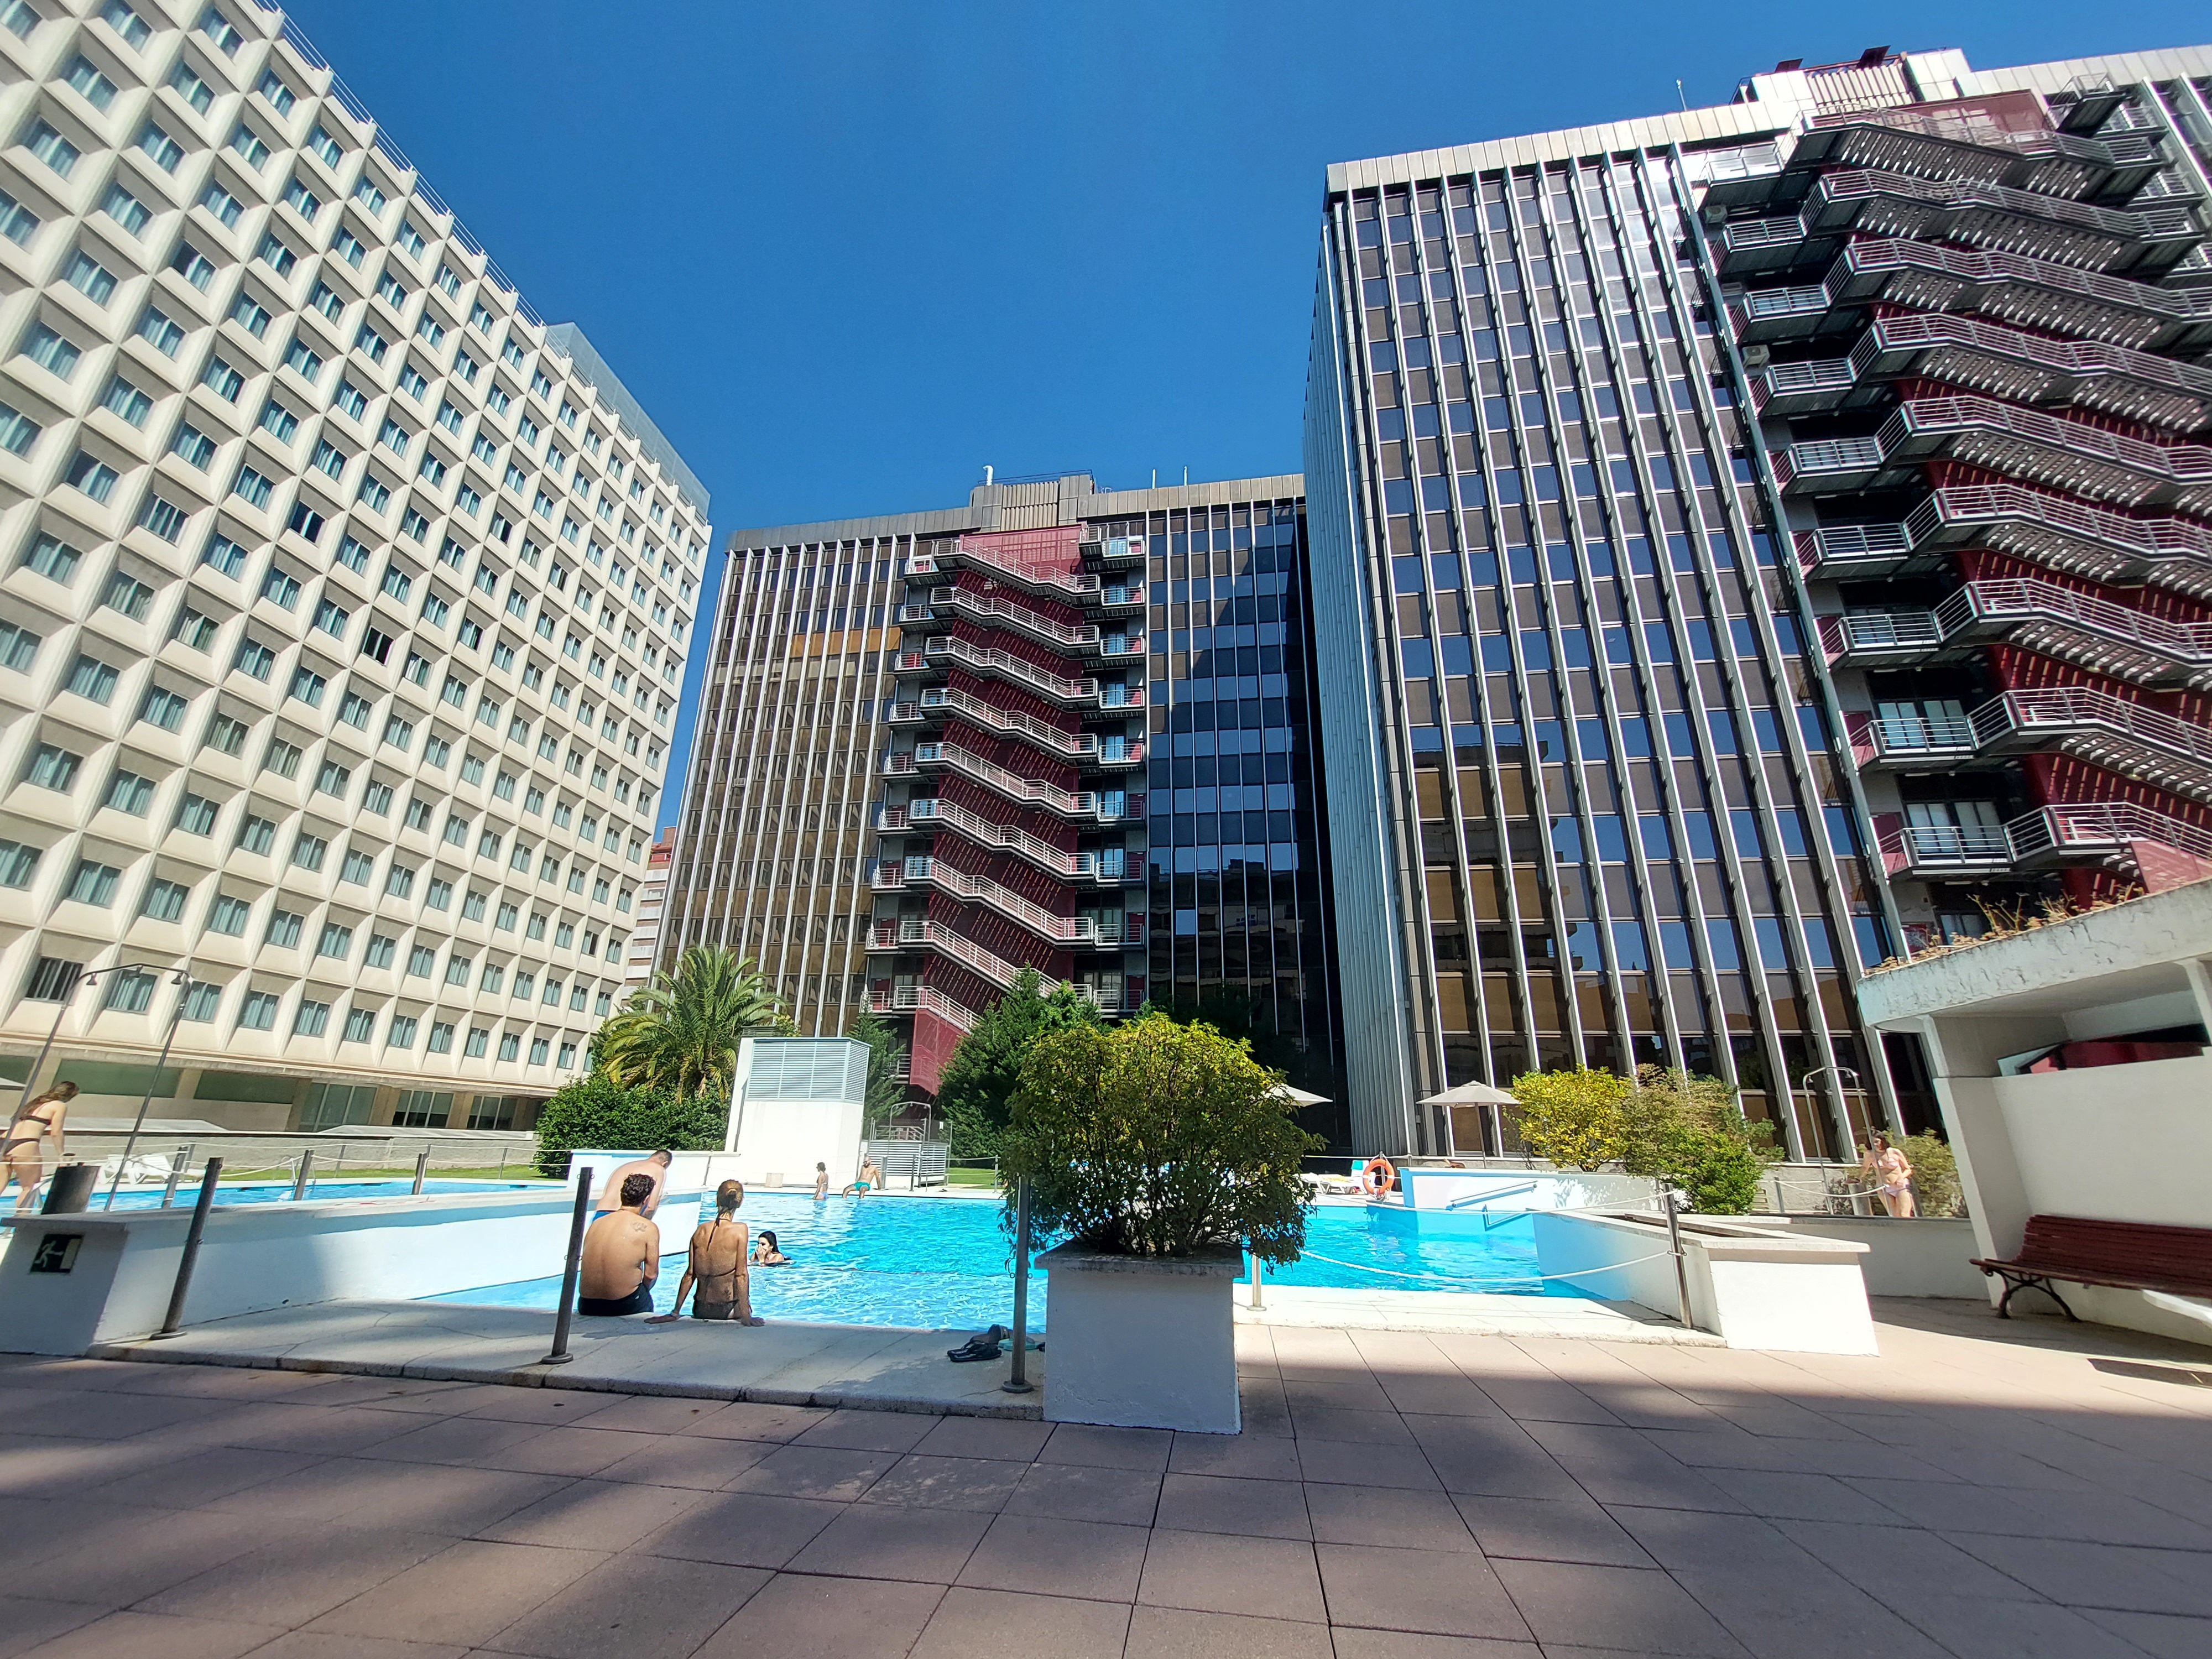
\includegraphics[scale=0.05]{Figures/pool.jpg}
    \end{figure}
    \end{textblock*}
    
    \begin{textblock*}{4.0cm}(7.5cm,.8cm)
    \begin{figure}
        \centering
        \includegraphics[scale=0.02,angle=-90,origin=c]{Figures/entrecote.jpg}
    \end{figure}
    \end{textblock*}
    
    
    \begin{textblock*}{3.0cm}(11.5cm,.8cm)
    \begin{figure}
        \centering
        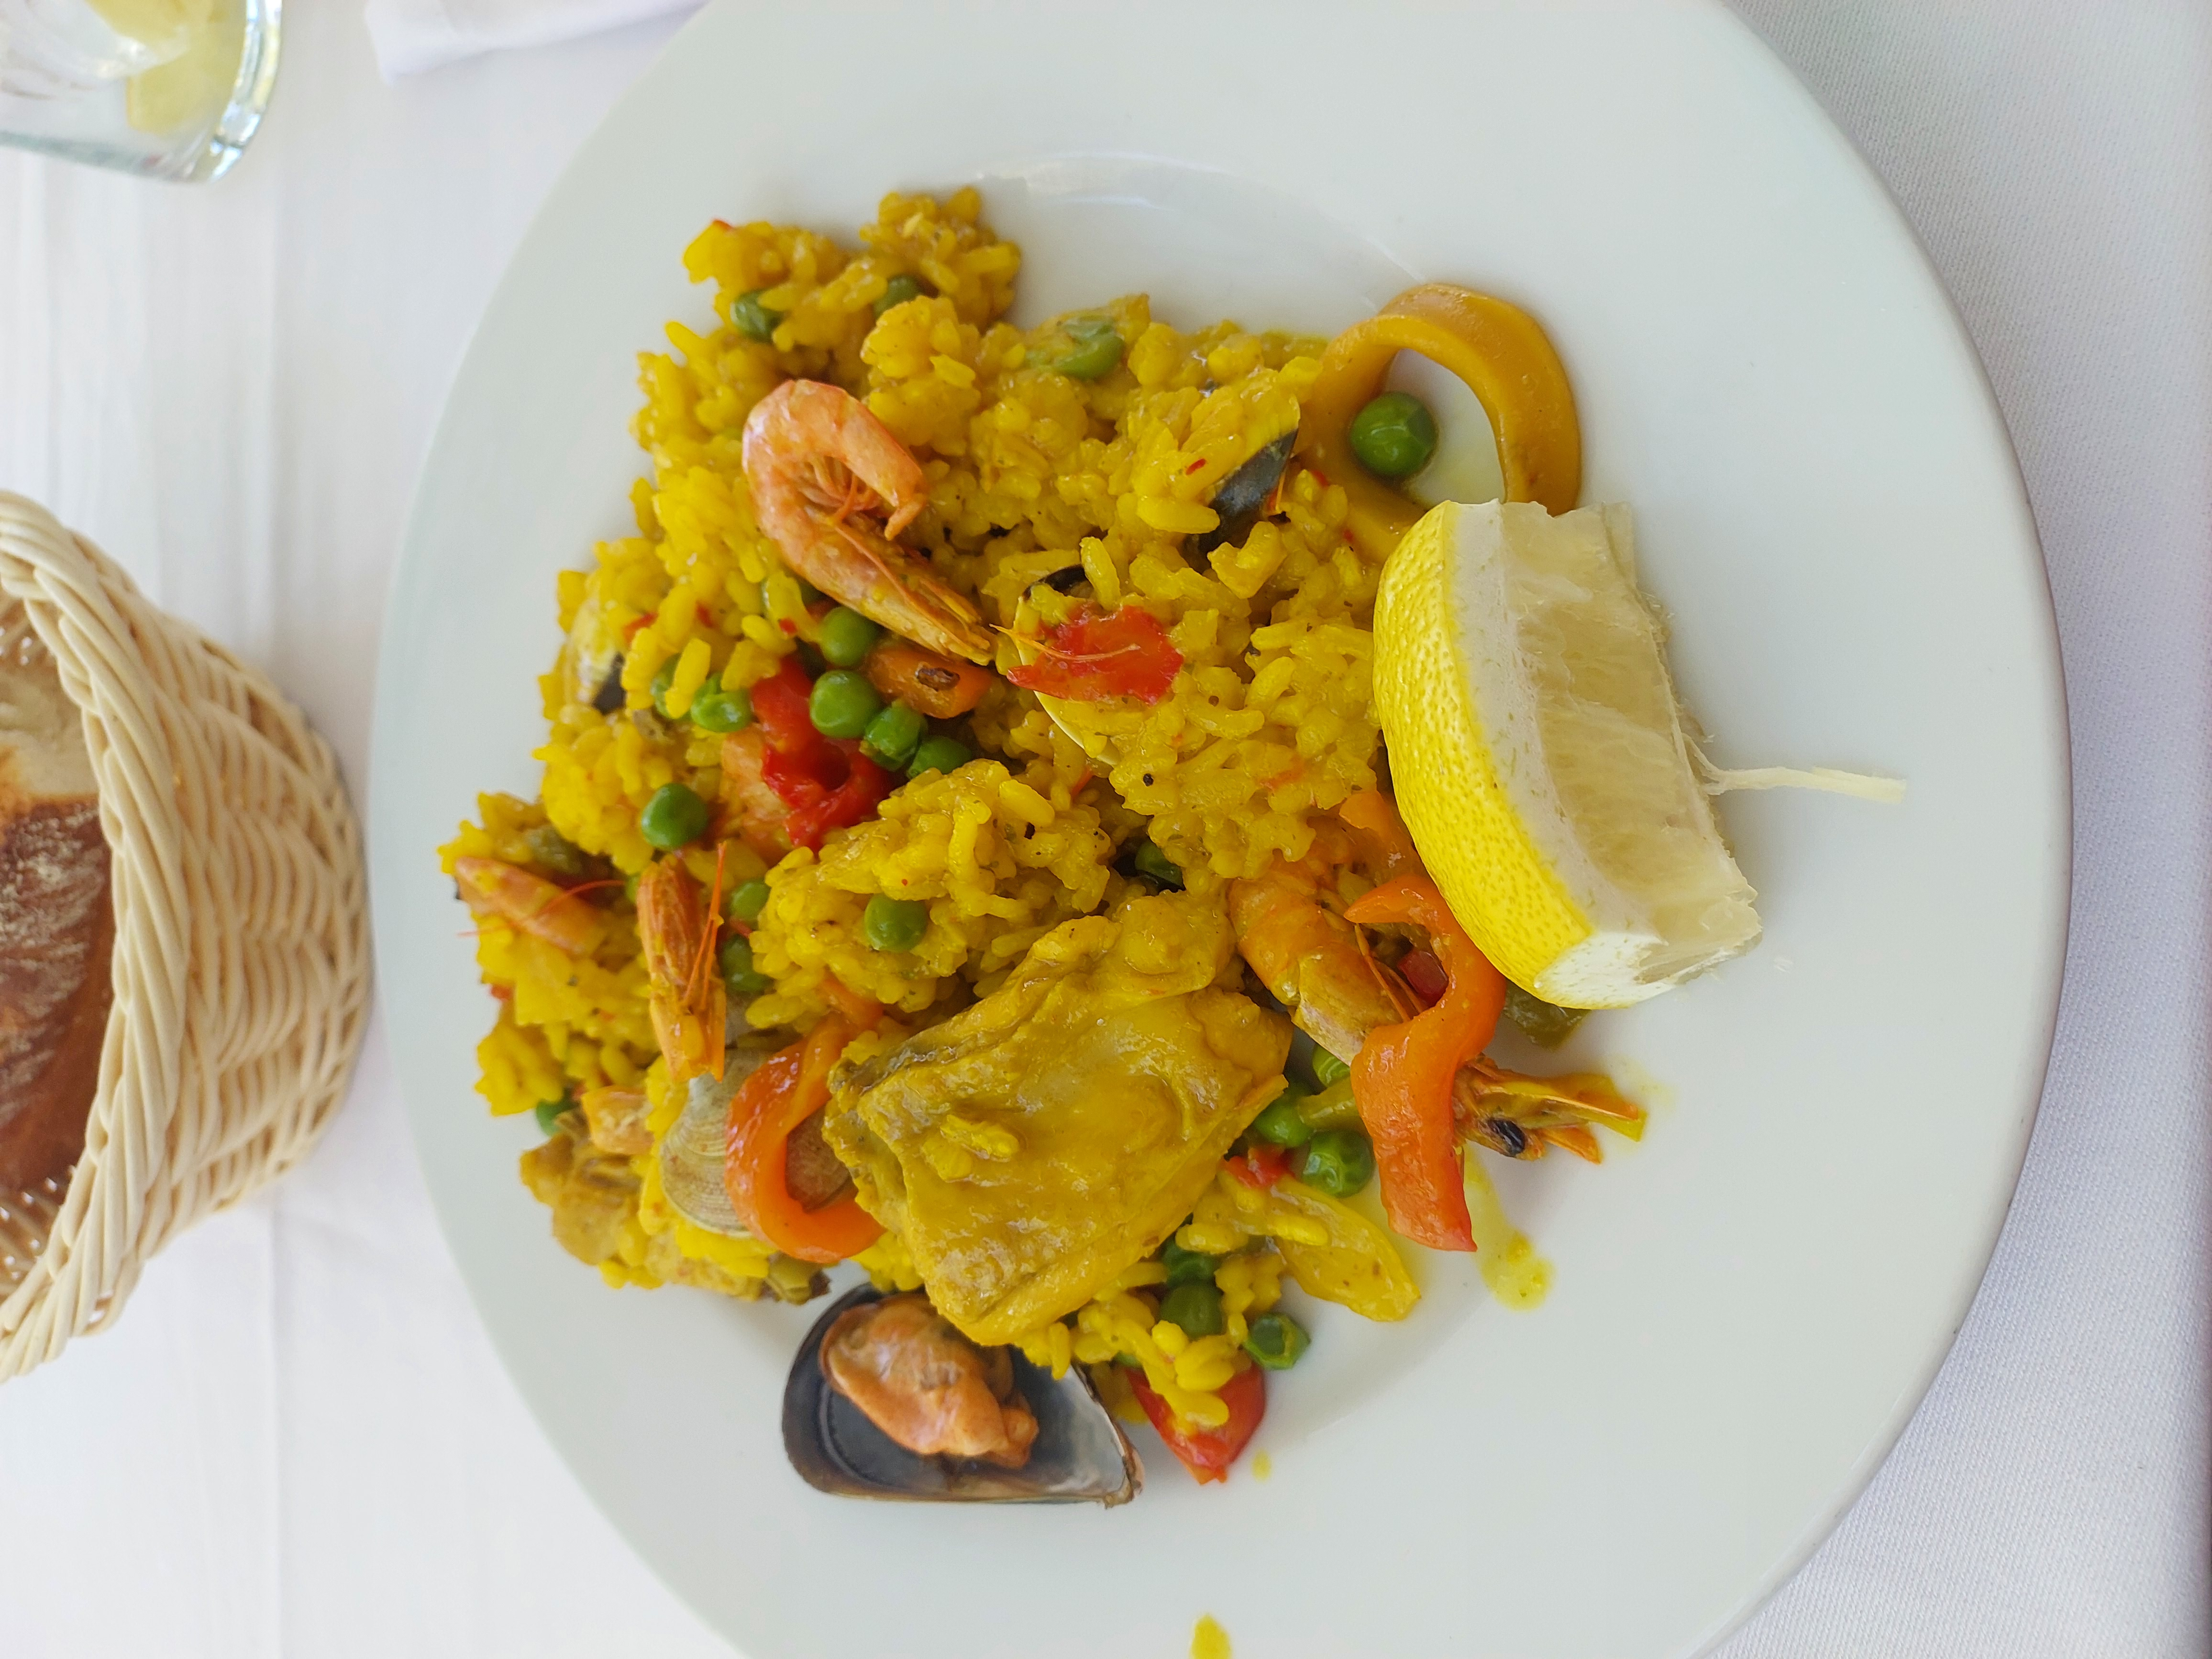
\includegraphics[scale=0.02,angle=-90,origin=c]{Figures/paella.jpg}
    \end{figure}
    \end{textblock*}
    
    \begin{textblock*}{4.0cm}(9cm,4.5cm)
    \begin{figure}
        \centering
    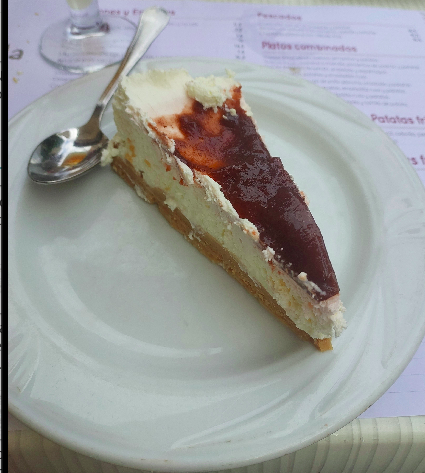
\includegraphics[scale=0.15]{Figures/cake.png}
    \end{figure}
    \end{textblock*}}
    
    
    \end{frame}
    

%%%%%%%%%%%%%%%%%%%%%%%%%%%%%%%%%%%%%%%%%%%%%%%%%%%

\begin{frame}{Outline}
  \tableofcontents
\end{frame}

% \begin{frame}{Outline}
% \tableofcontents[currentsection]

% \begin{textblock*}{10.0cm}(.2cm,1.2cm)
% \begin{itemize}
% \item Hexagonal boron nitride (hBN) in polaritonics
% ~\\

% \item hBN and setup
% ~\\

% \item hBN under an external periodic potential
% ~\\

% \item Excitonic problem
% \begin{itemize}
% \item Wannier equation and variational method
% \item Binding energies and wavefunctions
% \end{itemize}

% \item Optical response
% \begin{itemize}
% \item Conductivity
% \item Absorption
% \end{itemize}

% \item Polaritonics
% \begin{itemize}
% \item Conductivity
% \item Absorption
% \end{itemize}

% \item Summary


% \end{itemize}
% \end{textblock*}
% \end{frame}


\section{Screening}
%%%%%%%%%%%%%%%%%%%%%%%%%%%%%%%%%%%%%%%%%%%%%%%%%%%%%%%%%%%%%%%%%%%%

\begin{frame}{Outline}
    \tableofcontents[currentsection]
\end{frame}

\subsection{Screening (what is it?)}

\begin{frame}{Outline}
    \tableofcontents[currentsubsection]
\end{frame}

\begin{frame}{Screening...}

\begin{columns}[T]

\column{.5\linewidth}

\only<1->{
% \begin{textblock*}{5.0cm}(0cm,1.cm)
% \centering
% \textbf{...in an atom.}
% \end{textblock*}
% \begin{textblock*}{5.0cm}(3.4cm,1.5cm)
% \centering
% (Bare) Coulomb potential
% \begin{equation*}
%     v_c = \frac{Z e^2}{r}
% \end{equation*}
% \end{textblock*}


\textbf{...in an atom.} \\

(Bare) Coulomb potential $ v_c = \frac{Z e^2}{r}$

%\begin{textblock*}{5.0cm}(1cm,3.cm)
\begin{center}
    \centering
    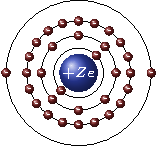
\includegraphics[width=0.4\textwidth]{Figures/atom.pdf} \hspace*{2cm}
\end{center}
%\end{textblock*}
    
}

% \begin{textblock*}{5.0cm}(0.2cm,1.5cm)
% \begin{figure}
%     \centering
%     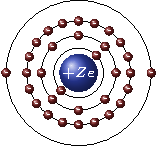
\includegraphics[scale=1.0]{Figures/atom.pdf}
% \end{figure}
% \end{textblock*}




\onslide<2->{
% \begin{textblock*}{5.0cm}(0.2cm,4.5cm)
% \begin{equation*}
%     Z_{\text{eff}} = Z - \tikzmark{a}\onslide<2->{{}\sigma}
% \end{equation*}
% \begin{tikzpicture}[remember picture,overlay]
% \onslide<3->{%
% \ColorBox[xshift=4cm,yshift=-1.2cm]{Phys. Rev. 36, 57, J.C. Slater}
% \draw[red!70!black,->] 
%   (box1) |- ([xshift=6pt,yshift=5pt]a.south east);
% }
% \end{tikzpicture}
% \begin{equation*}
%     W < v_c
% \end{equation*}
% \end{textblock*}
\vspace*{-0.7cm}
\begin{equation*}
    Z_{\text{eff}} = Z - \tikzmark{a}\onslide<2->{{}\sigma} \hspace*{1.8cm}
\end{equation*}
\begin{tikzpicture}[remember picture,overlay]
\onslide<3->{%
\ColorBox[xshift=5.5cm,yshift=-1.2cm]{Phys. Rev. 36, 57, J.C. Slater}
\draw[red!70!black,->] 
  (box1) |- ([xshift=6pt,yshift=5pt]a.south east);
}
\end{tikzpicture} 
\begin{equation*}
    W < v_c \hspace*{1.8cm}
\end{equation*}

}

\onslide<4->{
\column{.5\linewidth}

\textbf{...in a plasma.} $\phi(r) \propto e^{- \lambda_D r} / r\,, \lambda_D^2 = \varepsilon_r \varepsilon_0 k_B T /n q^2$



\begin{figure}
    \centering
    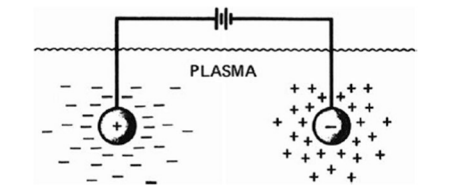
\includegraphics[scale=0.2]{Figures/Debye_shielding.png}
\end{figure}
\small{"Intro. to Plasma Physics and Controlled Fusion", F.F. Chen}
}

\onslide<5->{
\vspace*{-0.1cm}
\textbf{...in a crystal.}

\begin{figure}
    \centering
    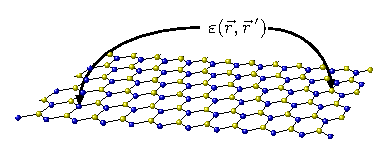
\includegraphics[scale=1.]{Figures/hBN_permittivity.pdf}
\end{figure}
}

\end{columns}


\end{frame}

%%%%%%%%%%%%%%%%%%%%%%%%%%%%%%%%%%
\subsection{The dielectric function}


%%%%%%%%%%%%%%%%%%%%%%%%%%%%%%%%%%%%%%%%%%%%%%%%%%%%%%%
\begin{frame}{Outline}
    \tableofcontents[currentsubsection]
\end{frame}
%%%%%%%%%%%%%%%%%%%%%%%%%%%%%%%%%%%%%%%%%%%%%%%%%%%%%%%%%%%%%%


\begin{frame}{The dielectric function: technical contexts}

\begin{columns}[T]

\column{.5\linewidth}


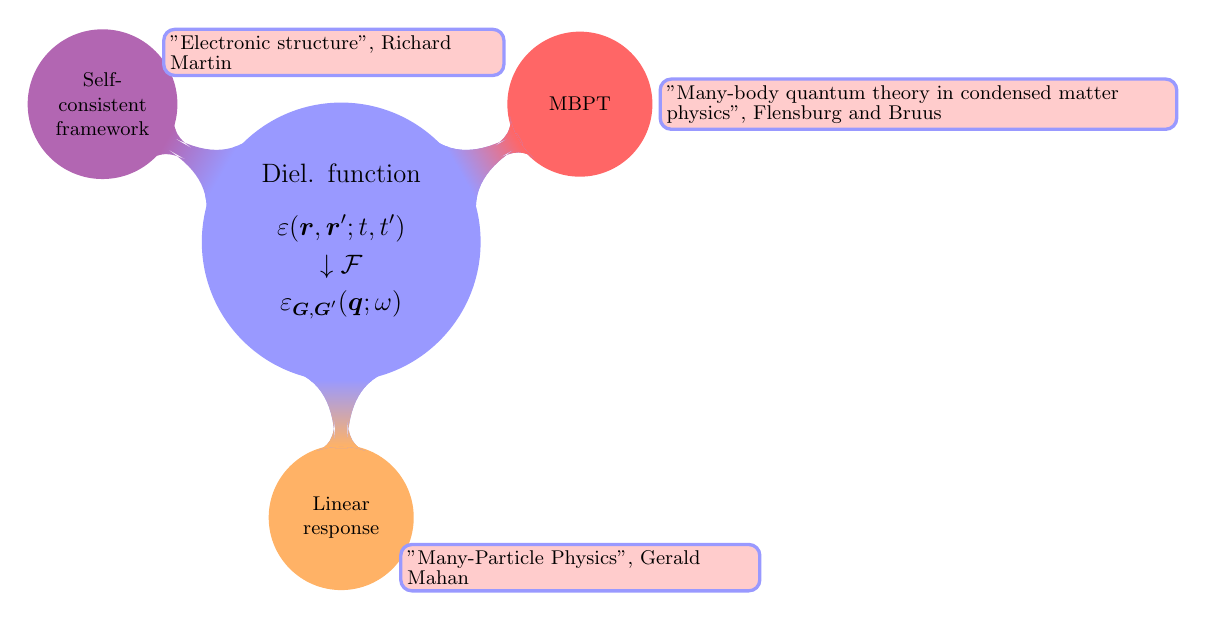
\begin{tikzpicture}[mindmap, grow cyclic, every node/.style=concept, concept color=blue!40!white,
    level 1/.append style={level distance=3.5cm,sibling angle=120},
    level 2/.append style={level distance=2.8cm,sibling angle=45},
    level 3/.append style={level distance=2cm,sibling angle=40},
    every annotation/.style={fill=red!20}]
    \tikzset{every node/.append style={scale=0.8}}
\node [concept] (dielefunc) { Diel. function 
\begin{gather*}
    \varepsilon(\vectormath{r},\vectormath{r}';t,t') \\
                           \downarrow \mathcal{F}    \\
    \varepsilon_{\vectormath{G},\vectormath{G}'}(\vectormath{q};\omega)
\end{gather*}}
    child [concept color = violet!60!white,grow=150] { node[alt=<{2}>{circular glow={fill=brass}}{}] (tdpt) {Self-consistent framework} }
    child [grow=30] {
    node[concept color = red!60!white,alt=<{4,5}>{circular glow={fill=brass}}{}] (mbpt) {MBPT} }
    child [grow=-90] {
    node[concept color = orange!60!white,alt=<{6,7}>{circular glow={fill=brass}}{}] (linres) {Linear response} };
    \node [annotation,right,text width=5.2cm, minimum width = 5.2cm,visible on=<3->] at (tdpt.north east)
        {\small "Electronic structure", Richard Martin};
    \path (dielefunc) to[circle connection bar switch color=from (blue!40!white) to (red!60!white)] (mbpt);
    \node [annotation,right,text width=8.cm, minimum width = 8.cm,visible on=<5->] at (mbpt.east)
        {\small "Many-body quantum theory in condensed matter physics", Flensburg and Bruus};
    \path (dielefunc) to[circle connection bar switch color=from (blue!40!white) to (orange!60!white)] (linres);
    \node [annotation,right,text width=5.5cm, minimum width = 5.5cm,visible on=<7>] at (linres.south east)
        {\small "Many-Particle Physics", Gerald Mahan};
\end{tikzpicture}



\column{.5\linewidth}

\only<6->{
\begin{textblock*}{8.0cm}(7.6cm,3.5cm)
"Quantum Theory of the Dielectric Constant in Real Solids", S.L. Adler, Phys. Rev. 126, 1962

\begin{figure}
    \centering
    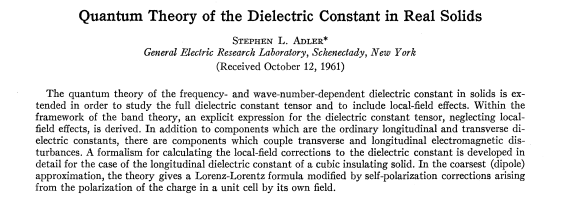
\includegraphics[scale=0.4]{Figures/Adlerspaper.png}
\end{figure}

\end{textblock*}}
    
\end{columns}

    
\end{frame}
%%%%%%%%%%%%%%%%%%%%%%%%%%%%%%%%%%%%%%%%%%%%%%%%%%%%%%%%%%%%%%%%%%%%%%%%%%%%%%%%%%%%%%%%%%%%%%%%


\begin{frame}{The dielectric function: full and non-interacting}

"Interacting Electrons:
Theory and Computational Approaches", Richard Martin et. al, 2016
\vspace{-0.2cm}
\begin{equation*}
    \varepsilon^{-1}(\vectormath{r},\vectormath{r}';t,t') = \delta(\vectormath{r}-\vectormath{r}') \delta(t-t') + \int \dr'' \int_{-\infty}^t \dif t'' \chi(\vectormath{r},\vectormath{r}';t-t'') v_c(\vectormath{r}-\vectormath{r}') 
\end{equation*}

\onslide<2->{
\begin{equation*}
    \varepsilon^{\text{RPA}}(\vectormath{r},\vectormath{r}';t,t') = \delta(\vectormath{r}-\vectormath{r}') \delta(t-t') - \int \dr'' \int_{-\infty}^t \dif t'' \chi^0(\vectormath{r},\vectormath{r}';t-t'') v_c(\vectormath{r}-\vectormath{r}') 
\end{equation*}
}


\onslide<3->{
\vspace{-0.2cm}
Hedin's equations: ($(1,2) \equiv (\vectormath{r}_1,t_1;\vectormath{r}_2,t_2)$, f.egs.)
\vspace{-0.1cm}
\begin{align*}
    W (1,2) &= v_c (1,2) + \int \dif3 \dif4 v_c (1,3) P(3,4) W(4,2) \text{   (Dyson's eq.)}\\
    P(1,2) &= -i \int \dif3  \dif4\, G(1,3) G(4,1^+) \Gamma(3,4;2) \\
    \Sigma(1,2) &= \int \dif3 \dif4\, G(1,3) \Gamma(3,2;4) W(4,1^+) \\
    \Gamma(1,2;3) &= \delta(1,2) \delta(1,3) + \slidehcancel<4>{\int \dif4 \dif5 \dif6 \dif7 \, \frac{\delta \Sigma(1,2)}{\delta G(4,5)} G(4,6) G(7,5)  \Gamma(6,7;3)} \,,
\end{align*}
}

    
\end{frame}

%%%%%%%%%%%%%%%%%%%%%%%%%%%%%%%%%%%%%%%%%%%

\begin{frame}{The dielectric function: $GW$ and RPA}
"Interacting Electrons:
Theory and Computational Approaches", Richard Martin et. al, 2016
\vspace{-0.2cm}
\begin{equation*}
    \varepsilon^{-1}(\vectormath{r},\vectormath{r}';t,t') = \delta(\vectormath{r}-\vectormath{r}') \delta(t-t') + \int \dr'' \int_{-\infty}^t \dif t'' \chi(\vectormath{r},\vectormath{r}';t-t'') v_c(\vectormath{r}-\vectormath{r}') 
\end{equation*}


\begin{equation*}
    \varepsilon^{\text{RPA}}(\vectormath{r},\vectormath{r}';t,t') = \delta(\vectormath{r}-\vectormath{r}') \delta(t-t') - \int \dr'' \int_{-\infty}^t \dif t'' \chi^0(\vectormath{r},\vectormath{r}';t-t'') v_c(\vectormath{r}-\vectormath{r}') 
\end{equation*}


Hedin's equations: ($(1,2) \equiv (\vectormath{r}_1,t_1;\vectormath{r}_2,t_2)$, f.egs.)
\vspace{-0.2cm}
\begin{align*}
    W (1,2) &= v_c (1,2) + \int \dif3 \dif4 v_c (1,3) P^0(3,4) W(4,2) \\
    P^0(1,2) &= -i \int \dif3\, G(1,3) G(3,2) \text{, Random Phase Approximation} \\
    \Sigma(1,2) &= \int \dif3\, G(1,3) W(3,2) \text{, $GW$ approximation} \\
    \Gamma(1,2;3) &= \delta(1,2) \delta(1,3) + \hcancel{\int \dif4 \dif5 \dif6 \dif7 \, \frac{\delta \Sigma(1,2)}{\delta G(4,5)} G(4,6) G(7,5)  \Gamma(6,7;3)} \,,
\end{align*}


\end{frame}

%%%%%%%%%%%%%%%%%%%%%%%%%%%%%%%%%%%%%%%%%%%%%%%%%%

\section{The screened potential}

%%%%%%%%%%%%%%%%%%%%%%%%%%%%%%%%%%%%%%%%%%%%%%%%%%
\begin{frame}{Outline}
    \tableofcontents[currentsection]
\end{frame}


\subsection{RPA polarizability: useful expressions}

%%%%%%%%%%%%%%%%%%%%%%%%%%%%%%%%%%%%%%%%%%%%%%%%%%
\begin{frame}{Outline}
    \tableofcontents[currentsubsection]
\end{frame}

\begin{frame}{RPA polarizability: general expression}

% \begin{columns}[T]

% \column{.5\linewidth}

\onslide<1->{
\begin{equation*}
    \chi_0 (\vectormath{r},\vectormath{r}';\omega) = \sum_{i,j} (f_i - f_j) \frac{\phi_i^*(\vectormath{r}) \phi_j(\vectormath{r}) \phi_j^*(\vectormath{r}') \phi_i(\vectormath{r}')}{\epsilon_i - \epsilon_j + \hw + \ii \hbar \alpha}
\end{equation*}
}

\onslide<2->{
\begin{equation*}
    \chi_0 (\vectormath{r},\vectormath{r}';\omega) = \sum_{v \vectormath{k}, c\vectormath{k}'} \left[ \frac{\psi_{c \vectormath{k}'}(\vectormath{r}) \psi_{v \vectormath{k}}^*(\vectormath{r}) \psi_{v \vectormath{k}}(\vectormath{r}') \psi_{c \vectormath{k}'}^*(\vectormath{r}') }{\hw -(\epsilon_{c \vectormath{k}'} - \epsilon_{v \vectormath{k}})   + \ii \hbar \alpha} - \frac{ \psi_{v \vectormath{k}}(\vectormath{r}) \psi_{c \vectormath{k}'}^*(\vectormath{r}) \psi_{c \vectormath{k}'}(\vectormath{r}') \psi_{v \vectormath{k}}^*(\vectormath{r}') }{\hw + (\epsilon_{c \vectormath{k}'} - \epsilon_{v \vectormath{k}}) + \ii \hbar \alpha} \right]\,.
\end{equation*}

\begin{equation*}
    \braket{\vectormath{r}}{n, \vectormath{k}} = \psi_{n \vectormath{k}}(\vectormath{r})\,, \alpha \to 0^+
\end{equation*}

\begin{equation*}
    \psi_{n \bk} (\br) = \frac{1}{\sqrt{N}} \sum_{\bR} \ee^{\ii \bk \cdot \bR} \sum_{i \alpha} C_{i \alpha}^{n \bk} \phi_{\alpha} (\br - \bR - \bt_i)\, \text{, in the TB approx.}
\end{equation*}
}
%\end{columns}
    
\end{frame}

\begin{frame}{RPA polarizability: momentum space}

% \begin{columns}[T]

% \column{.5\linewidth}

\begin{align*}
     \chi^0 (\br,\br';\omega) &= \frac{1}{N} \sum_{\bq,\bq'} \ee^{\ii \bq \cdot \br} \chi^0(\bq,\bq';\omega) \ee^{-\ii \bq' \cdot \br'} \onslide<2->{= \\
     &= \frac{1}{N} \sum_{\bq} \sum_{\bG'} \ee^{\ii \bq \cdot (\br - \br')}  \ee^{-\ii \bG' \cdot \br'} \chi^0(\bq,\bq + \bG';\omega)} \onslide<3->{= \\
     &=\frac{1}{N}  \sum_{\bq \in \mathrm{BZ}} \sum_{\bG,\bG'} \ee^{\ii \bq \cdot (\br - \br')} \ee^{\ii \bG \cdot \br} \ee^{-\ii( \bG' + \bG ) \cdot \br'} \chi^0(\bq + \bG,\bq + \bG + \bG';\omega) = \\
     &=\frac{1}{N}  \sum_{\bq \in \mathrm{BZ}} \sum_{\bG,\bG'} \ee^{\ii \bq \cdot (\br - \br')} \ee^{\ii \bG \cdot \br} \ee^{-\ii \bG' \cdot \br'} \underbrace{\chi^0(\bq + \bG,\bq + \bG';\omega)}_{\chi^0_{\bG,\bG'}(\bq;\omega)}\,,}
\end{align*}

 \onslide<4->{
\begin{equation*}
    \chi^0_{\bG \bG'} (\bq;\omega) = \int \dr \int \dr' \ee^{-\ii(\bq + \bG) \cdot \br} \chi_0 (\vectormath{r},\vectormath{r}';\omega) \ee^{\ii(\bq + \bG') \cdot \br}
\end{equation*}}

%\end{columns}
    
\end{frame}



\begin{frame}{Static RPA polarizability: $\br$ and $\bq$ spaces}

\begin{equation*}
    \chi_0 (\vectormath{r},\vectormath{r}';\omega) = \sum_{v \vectormath{k}, c\vectormath{k}'} \left[ \frac{\psi_{c \vectormath{k}'}(\vectormath{r}) \psi_{v \vectormath{k}}^*(\vectormath{r}) \psi_{v \vectormath{k}}(\vectormath{r}') \psi_{c \vectormath{k}'}^*(\vectormath{r}') }{\hw -(\epsilon_{c \vectormath{k}'} - \epsilon_{v \vectormath{k}})   + \ii \hbar \alpha} - \frac{ \psi_{v \vectormath{k}}(\vectormath{r}) \psi_{c \vectormath{k}'}^*(\vectormath{r}) \psi_{c \vectormath{k}'}(\vectormath{r}') \psi_{v \vectormath{k}}^*(\vectormath{r}') }{\hw + (\epsilon_{c \vectormath{k}'} - \epsilon_{v \vectormath{k}}) + \ii \hbar \alpha} \right]\,.
\end{equation*}

\begin{equation*}
    \chi_0 (\vectormath{r},\vectormath{r}') = - \sum_{v \vectormath{k}, c\vectormath{k}'} \frac{ 2 \Re{\psi_{c \vectormath{k}'}(\vectormath{r}) \psi_{v \vectormath{k}}^*(\vectormath{r}) \psi_{v \vectormath{k}}(\vectormath{r}') \psi_{c \vectormath{k}'}^*(\vectormath{r}')} }{\epsilon_{c \vectormath{k}'} - \epsilon_{v \vectormath{k}}}
\end{equation*}

\begin{equation*}
    \chi^0_{\bG \bG'} (\bq;\omega) = \frac{1}{\Omega} \sum_{n,n'} \sum_{\bk} (f_{n,\bk + \bq} - f_{n',\bk}) \frac{\bra{n,\bk + \bq} \ee^{\ii(\bq + \bG) \cdot \br} \ket{n',\bk} \bra{n',\bk} \ee^{-\ii(\bq + \bG') \cdot \br} \ket{n,\bk + \bq}}{\epsilon_{n,\bk + \bq} - \epsilon_{n',\bk} + \hw + \ii \hbar \alpha}
\end{equation*}


\begin{equation*}
  \chi^0_{\bG \bG'} (\bq) = \frac{1}{\Omega} \sum_{n}^{\text{occ}} \sum_{n'}^{\text{emp}} \sum_{\bk} \frac{\bra{n,\bk + \bq} \ee^{\ii(\bq + \bG) \cdot \br} \ket{n',\bk} \bra{n',\bk} \ee^{-\ii(\bq + \bG') \cdot \br} \ket{n,\bk + \bq}}{\epsilon_{n,\bk + \bq} - \epsilon_{n',\bk} }
\end{equation*}
    
\end{frame}


\subsection{RPA dielectric function and screened potential}

%%%%%%%%%%%%%%%%%%%%%%%%%%%%%%%%%%%%%%%%%%%%%%%%%%
\begin{frame}{Outline}
    \tableofcontents[currentsubsection]
\end{frame}


\begin{frame}{RPA dielectric function}

\onslide<1->{
\begin{equation*}
    \varepsilon^{\text{RPA}}(\vectormath{r},\vectormath{r}';t,t') = \delta(\vectormath{r}-\vectormath{r}') \delta(t-t') - \int \dr'' \int_{-\infty}^t \dif t'' \chi^0(\vectormath{r},\vectormath{r}';t-t'') v_c(\vectormath{r}-\vectormath{r}') 
\end{equation*}}

\onslide<2->{
\begin{equation*}
    \varepsilon_{\bG \bG'} (\bq) = \delta_{\bG \bG'} - v_c(\bq + \bG) \chi^0_{\bG \bG'} (\bq)\,, v_c(\bq) = \frac{e^2}{2 \varepsilon_0 |\bq|}
\end{equation*}
}

\onslide<3->{
\begin{equation*}
  \chi^0_{\bG \bG'} (\bq) = \frac{1}{\Omega} \sum_{v,c} \sum_{\bk} \frac{\bra{v,\bk + \bq} \ee^{\ii(\bq + \bG) \cdot \br} \ket{c,\bk} \bra{c,\bk} \ee^{-\ii(\bq + \bG') \cdot \br} \ket{v,\bk + \bq}}{\epsilon_{v,\bk + \bq} - \epsilon_{c,\bk} } \text{see [1]}
\end{equation*}

[1] Jack Deslippe et al., “BerkeleyGW: A massively parallel computer package for the calculation of the quasiparticle and optical properties of materials and nanostructures”, Computer Physics Communications 183.6 (2012)}

\end{frame}

\begin{frame}{The (RPA) screened electrostatic potential}

\onslide<1->{
\begin{equation*}
\begin{aligned}
    W(\br,\br') &= \int \dr'' \varepsilon^{-1} (\br,\br'')v_c (\br'',\br') \\
    W_{\bG,\bG'}(\bq) &= \varepsilon^{-1}_{\bG \bG'} (\bq) v_c(\bq+\bG')\,,
\end{aligned}
\end{equation*}}

\onslide<2->{
Ignoring local field effects ($\bG=\bG'=0$) and defining $\varepsilon_{\text{mac}}(\bq) = 1/\varepsilon^{-1}_{\bzero \bzero}(\bq)$

\begin{equation*}
    W(\bq) =  \frac{v_c(\bq)}{\varepsilon_{\text{mac}}(\bq)}\,,
\end{equation*}}

\onslide<3->{

For a 2D semiconductor/insulator $\varepsilon_{\text{mac}}(\bq) = \varepsilon_{\text{2D}}(\bq) \approx 1 + r_0 q \equiv \varepsilon_{\text{RK}}(\bq)$

\begin{equation*}
    V_{\text{RK}}(q) =  \frac{v_c(q)}{\varepsilon_{\text{RK}}(q)} = \frac{e^2}{2 \varepsilon_0 (1 + r_0 q) q}\,,
\end{equation*}}


\end{frame}


\section{Dielectric function in the Tight-Binding approximation}

%%%%%%%%%%%%%%%%%%%%%%%%%%%%%%%%%%%%%%%%%%%%%%%%%%%
\begin{frame}{Outline}
    \tableofcontents[currentsection]
\end{frame}

\subsection{Tight-Binding approximation}

%%%%%%%%%%%%%%%%%%%%%%%%%%%%%%%%%%%%%%%%%%%%%%%%%%%
\begin{frame}{Outline}
    \tableofcontents[currentsubsection]
\end{frame}

\begin{frame}{Bloch states in the TB approx.}

\onslide<1->{
In the linear combination of atomic orbitals (LCAO) method
\vspace{-0.1cm}
\begin{equation*}
    \psi_{n \bk} (\br) = \frac{1}{\sqrt{N}} \sum_{\bR} \ee^{\ii \bk \cdot \bR} \sum_{i \alpha} C_{i \alpha}^{n \bk} \phi_{\alpha} (\br - \bR - \bt_i)\,
\end{equation*}
}

\onslide<2->{
Frequently, we work under the tight-binding approximation: retain nearest neighbors and neglect overlap between orbitals. 
}
\vspace{-0.1cm}
\onslide<2->{
\begin{equation*}
    \psi_{n \bk} (\br) = \frac{1}{\sqrt{N}} \sum_{\bR_j} \psi_j(\bk) \Phi_{j} (\bk,\br)\,, \Phi_{j} (\bk,\br) = \ee^{\ii \bk \cdot \bR} \phi (\br - \bR - \bt_j)
\end{equation*}
}

\onslide<3->{
\vspace{-0.4cm}
\begin{equation*}
    H \psi_{n \bk} (\br) = E \psi_{n \bk} (\br) \Leftrightarrow \sum_j \psi_j(\bk) H \Phi_{j} (\bk,\br) = E \sum_j \psi_j(\bk) \Phi_{j} (\bk,\br) \,.
\end{equation*}}

\onslide<4->{
\vspace{-0.5cm}
\begin{equation*}
    \sum_j \psi_j(\bk) \underbrace{\int \dr\, \Phi^*_{i} (\bk,\br) H \Phi_{j} (\bk,\br)}_{H_{ij}(\bk)} = E \sum_j \psi_j(\bk) \underbrace{ \int \dr\, \Phi^*_{i} (\bk,\br)  \Phi_{j} (\bk,\br)}_{S_{ij}(\bk)}
\end{equation*}}

\end{frame}

\begin{frame}{Bloch Hamiltonian in the TB approx.}

\onslide<1->{
Defining $H_{ij}(\bk) = \mel{\Phi_{i} (\bk,\br)}{H}{\Phi_{j} (\bk,\br)}$ and $S_{ij}(\bk) = \braket{\Phi_{i} (\bk,\br)}{\Phi_{j} (\bk,\br)}$

\begin{equation*}
    \sum_j \psi_j(\bk) H_{ij}(\bk) = E \sum_j \psi_j(\bk) S_{ij}(\bk)
\end{equation*}}

\onslide<2->{
The transfer integral matrix elements read
\begin{equation*}
\begin{split}
    H_{ij}(\bk) &= \mel{\Phi_{i} (\bk,\br)}{H}{\Phi_{j} (\bk,\br)} =  \sum_{ij} \ee^{\ii \bk \cdot ( \bR_j - \bR_i)} \mel{\phi(\br - \bR - \bt_i)}{H}{\phi (\br - \bR - \bt_j)} = \\
    &= \sum_{\bR_j} \ee^{\ii \bk \cdot \bR_j} \mel{\phi_i (\br)}{H}{\phi_j (\br - \bR_j)} = \underbrace{\sum_{\bR_j} \ee^{\ii \bk \cdot \bR_j} H_{ij} (\bR_j)}_{\text{Bloch Ham.}}\,,  H (\bR_j) \to \text{Fock matrix at } \bR_j
\end{split} 
\end{equation*}}

\onslide<3->{
TB approx. $\Rightarrow S_{ij}(\bk) \approx \delta_{ij}$ and eigenvalue/eigenvector problem:
\begin{equation*}
    H(\bk) \psi(\bk) = E  \psi(\bk)
\end{equation*}}
    
\end{frame}

\begin{frame}{Tight-Binding coefficients}

\begin{columns}

\column{0.6\linewidth}

    
\begin{equation*}
    \psi_{n \bk} (\br) = \frac{1}{\sqrt{N}} \sum_{\bR} \ee^{\ii \bk \cdot \bR} \sum_{i \alpha} C_{i \alpha}^{n \bk} \phi_{\alpha} (\br - \bR - \bt_i)\,
\end{equation*}

\begin{equation*}
    H(\bk) \underline{C}^{n\bk} = \epsilon_{n\bk} \underline{C}^{n\bk}
\end{equation*}

\column{0.5\linewidth}

\begin{equation*}
    H(\bk) \begin{bmatrix}
C^{n\vectormath{k}}_{1,1} \\
C^{n\vectormath{k}}_{1,2} \\
\vdots \\
C^{n\vectormath{k}}_{1,N^1_{o}} \\
C^{n\vectormath{k}}_{2,1} \\
\vdots \\
C^{n\vectormath{k}}_{2,N^2_{o}} \\
\vdots \\
C^{n\vectormath{k}}_{N_a,N^{N_a}_{o}-1} \\
C^{n\vectormath{k}}_{N_a,N^{N_a}_{o}} 
\end{bmatrix} = \epsilon_{n\bk} \begin{bmatrix}
C^{n\vectormath{k}}_{1,1} \\
C^{n\vectormath{k}}_{1,2} \\
\vdots \\
C^{n\vectormath{k}}_{1,N^1_{o}} \\
C^{n\vectormath{k}}_{2,1} \\
\vdots \\
C^{n\vectormath{k}}_{2,N^2_{o}} \\
\vdots \\
C^{n\vectormath{k}}_{N_a,N^{N_a}_{o}-1} \\
C^{n\vectormath{k}}_{N_a,N^{N_a}_{o}}  
\end{bmatrix} 
\end{equation*}

\end{columns}

\end{frame}


\subsection{Dielectric function within TB}

%%%%%%%%%%%%%%%%%%%%%%%%%%%%%%%%%%%%%%%%%%%%%%%%%%%
\begin{frame}{Outline}
    \tableofcontents[currentsubsection]
\end{frame}

\begin{frame}{Polarizability in the TB approximation}

\begin{equation*}
    \psi_{n \bk} (\br) = \frac{1}{\sqrt{N}} \sum_{\bR} \ee^{\ii \bk \cdot \bR} \sum_{i \alpha} C_{i \alpha}^{n \bk} \phi_{\alpha} (\br - \bR - \bt_i)\,
\end{equation*}

\onslide<1->{
\begin{equation*}
\begin{split}
  \chi^0_{\bG \bG'} (\bq) &= \frac{1}{\Omega} \sum_{v,c} \sum_{\bk} \frac{\bra{v,\bk + \bq} \ee^{\ii(\bq + \bG) \cdot \br} \ket{c,\bk} \bra{c,\bk + \bq} \ee^{-\ii(\bq + \bG') \cdot \br} \ket{v,\bk}}{\epsilon_{v,\bk + \bq} - \epsilon_{c,\bk} } = \\
  &=\frac{1}{\Omega} \sum_{v,c} \sum_{\bk} \frac{M_{v c} (\bk,\bq,\bG) M^*_{v c} (\bk,\bq,\bG')}{\epsilon_{v,\bk + \bq} - \epsilon_{c,\bk} } \onslide<3->{= \frac{1}{A_{\text{UC}}N_k} \sum_{vc} \sum_{\bk} \frac{I^{\bG}_{v \bk + \bq, c \bk} (I^{\bG'}_{v \bk + \bq, c \bk})^*}{\epsilon_{v,\bk + \bq} - \epsilon_{c,\bk} }}
\end{split}
\end{equation*}}

\onslide<2->{
Point-like orbitals approximation $\phi^*_{\alpha} (\br - \bR - \bt_i) \phi_{\beta} (\br - \bR' - \bt_j) \approx \delta_{ij} \delta_{\alpha \beta} \delta_{\bR \bR'} \delta(\br - \bR - \bt_i)$:
\begin{equation*}
\begin{split}
  M_{n n'} (\bk,\bq,\bG) \equiv \bra{n,\bk +\bq} \ee^{\ii(\bq + \bG) \cdot \br} \ket{n',\bk} &= \int \dr\, \psi^*_{n,\bk + \bq} (\br) \ee^{\ii(\bq + \bG) \cdot \br} \psi_{n' \bk} (\br) = \\
  &= \sum_{i \alpha} (C_{i \alpha}^{n \bk+ \bq})^* C_{i \alpha}^{n' \bk}  \ee^{\ii (\bq + \bG)  \cdot \bt_i} \equiv I^{\bG}_{n \bk + \bq, n' \bk}
\end{split}
\end{equation*}}

\end{frame}



\begin{frame}{Dielectric function computation scheme}

\begin{enumerate}
    \item Diagonalize $H(\bk)$ and store all $\{\epsilon_{n\bk}\}$,$\{\underline{C}^{n\bk}\}$ in a BZ mesh \itemsep=2em
    \item Compute dielectric matrix $ \varepsilon_{\bG \bG'} (\bq) = \delta_{\bG \bG'} - v_c(\bq + \bG) \chi^0_{\bG \bG'} (\bq), \, \forall \bq \in \mathrm{BZ}$  \itemsep=2em
    \item Invert $\varepsilon_{\bG \bG'} (\bq) \,\forall \bq \in \mathrm{BZ}$ \itemsep=2em
    \item Compute $W_{\bG,\bG'}(\bq) = \varepsilon^{-1}_{\bG \bG'} (\bq) v_c(\bq+\bG') \, \forall \bq \in \mathrm{BZ}$ \itemsep=2em
    \item Compute the exciton (details for another time) \itemsep=2em
\end{enumerate}

\end{frame}


%%%%%%%%%%%%%%%%%%%%%%%%%%%%%%%%%%%%%%%%%
 
\section{Numerical results}

\begin{frame}{Outline}
    \tableofcontents[currentsection]
\end{frame}

%%%%%%%%%%%%%%%%%%%%%%%%%%%%%%%%%%%%%%%

\begin{frame}{Polarizability convergence}

\begin{columns}
    
\column{0.5\textwidth}

\begin{figure}[H]
\centering
\begin{subfigure}{.5\textwidth}
  \centering
  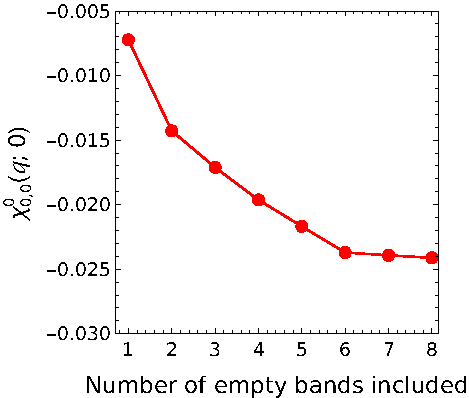
\includegraphics[width=1.0\linewidth]{Figures/Chi00MoS2TBq1.pdf}
\end{subfigure}%
\begin{subfigure}{.5\textwidth}
  \centering
    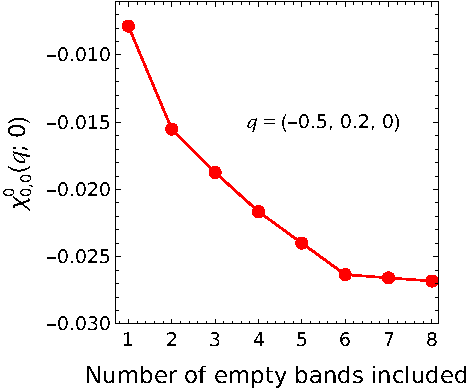
\includegraphics[width=1.0\linewidth]{Figures/Chi00MoS2TBq2.pdf}
\end{subfigure}
\caption{\ch{MoS2} tight-binding model by Ridolfi [1].}
\end{figure}

\column{0.5\textwidth}

\begin{figure}[H]
\centering
  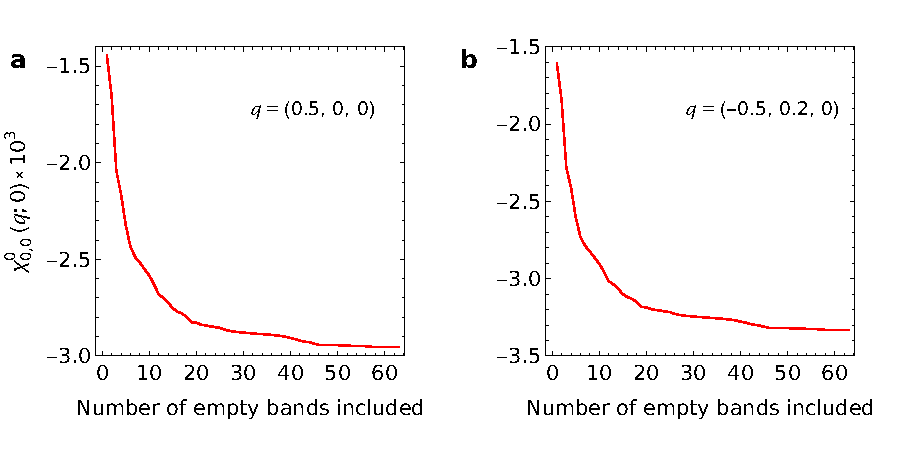
\includegraphics[width=1.0\linewidth]{Figures/Chi00hBNDFTq1&q2.pdf}
\caption{hBN, DFT (HSE06 
functional) using CRYSTAL [2].}
\end{figure}

\end{columns}


\begin{itemize}
    \item \relax [1] E. Ridolfi et al., Journal of Physics: Condensed Matter 27.36 (2015)
    \item \relax [2] A. Erba et al., Journal of Chemical Theory and Computation 19.20 (2023)
\end{itemize}
    
\end{frame}


\begin{frame}{Polarizability convergence: comparing models}

\begin{columns}
    
\column{0.5\textwidth}

\begin{figure}[H]
\centering
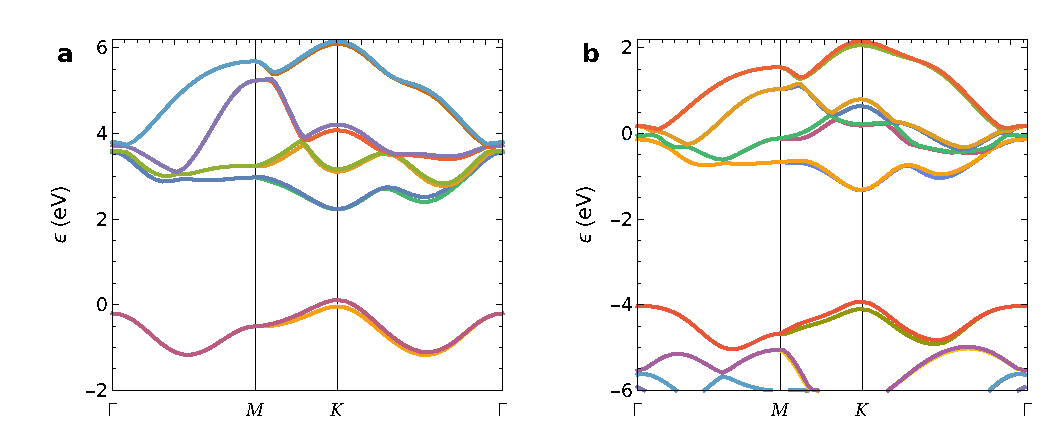
\includegraphics[width=1.\linewidth]{Figures/MoS2bandsTBvsWannier.pdf}
\caption{\ch{MoS2} bands, \textbf{a}-Ridolfi's TB model,  \textbf{b}-Wannier90 [1].}
\end{figure}

\column{0.5\textwidth}

\begin{figure}[H]
\centering
  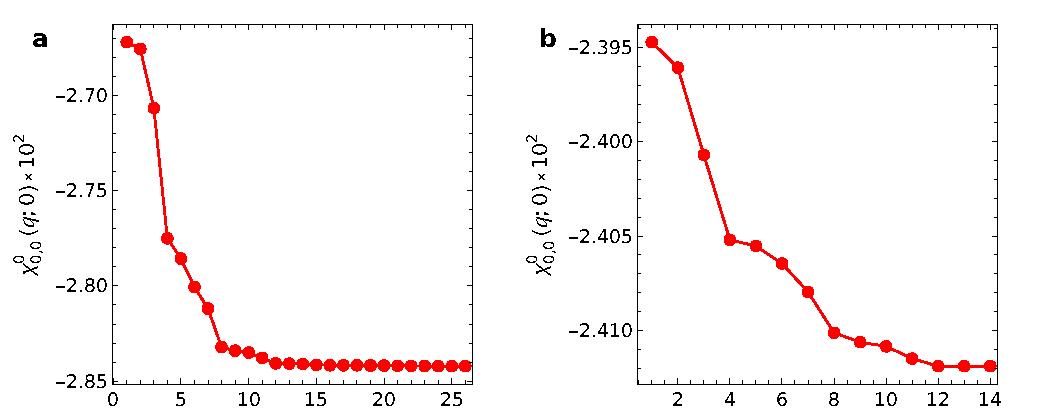
\includegraphics[width=1.0\linewidth]{Figures/Chi00MoS2TBvsWannierconverge.pdf}
\caption{$\chi_{\bzero \bzero} (\bq)$, $\bq=(0.5,0)$. (a->b, b->a)}
\end{figure}

\end{columns}

Convergence of the polarizability with the number of included valence bands, including all the conduction bands. Different values justified by a different band structure.


\begin{itemize}
    \item \relax [1] G. Pizzi et al., Journal of Physics: Condensed Matter 32.16 (2020)
\end{itemize}
    
\end{frame}


\begin{frame}{Polarizability in the Brillouin Zone}


\begin{figure}[H]
\centering
  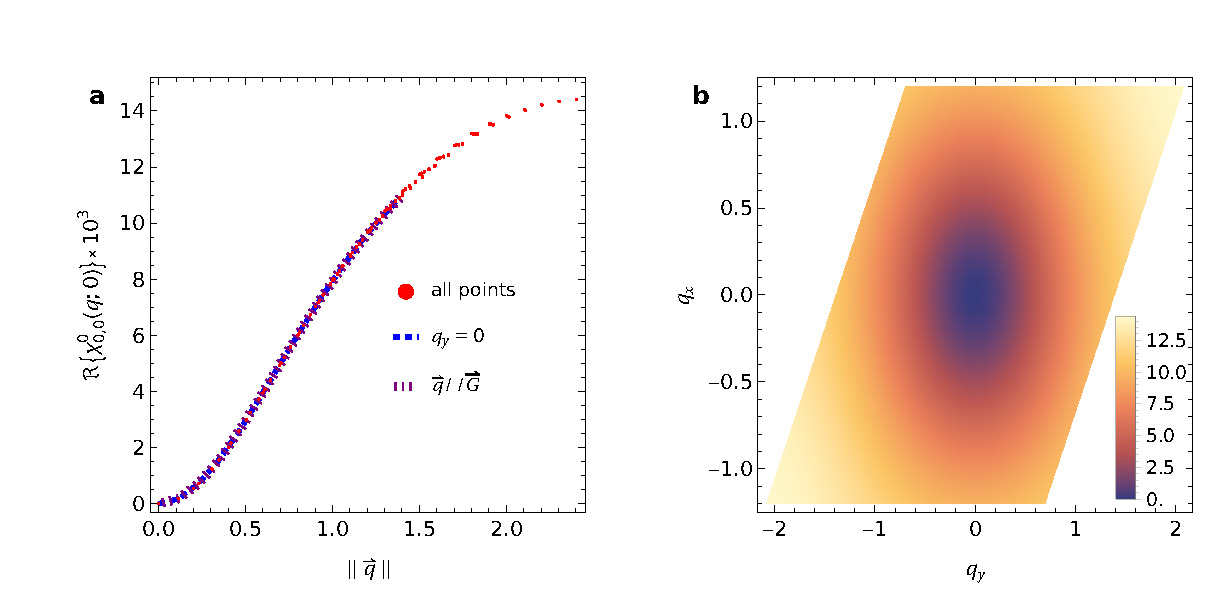
\includegraphics[width=0.8\linewidth]{Figures/Chi00hBNDFTmesh.pdf}
\caption{Panel \textbf{a}: $\chi^0_{\bzero \bzero} (\bq)$ vs. $|\bq|$; Panel \textbf{b}: $\chi^0_{\bzero \bzero} (\bq)$ vs. $\bq \in $ BZ. Calculation for hBN, whose bands were obtained within DFT with the HSE06 functional.}
\end{figure}
    
\end{frame}


\begin{frame}{Convergence of the inverse dielectric function}

\begin{figure}[h!]
    \centering
    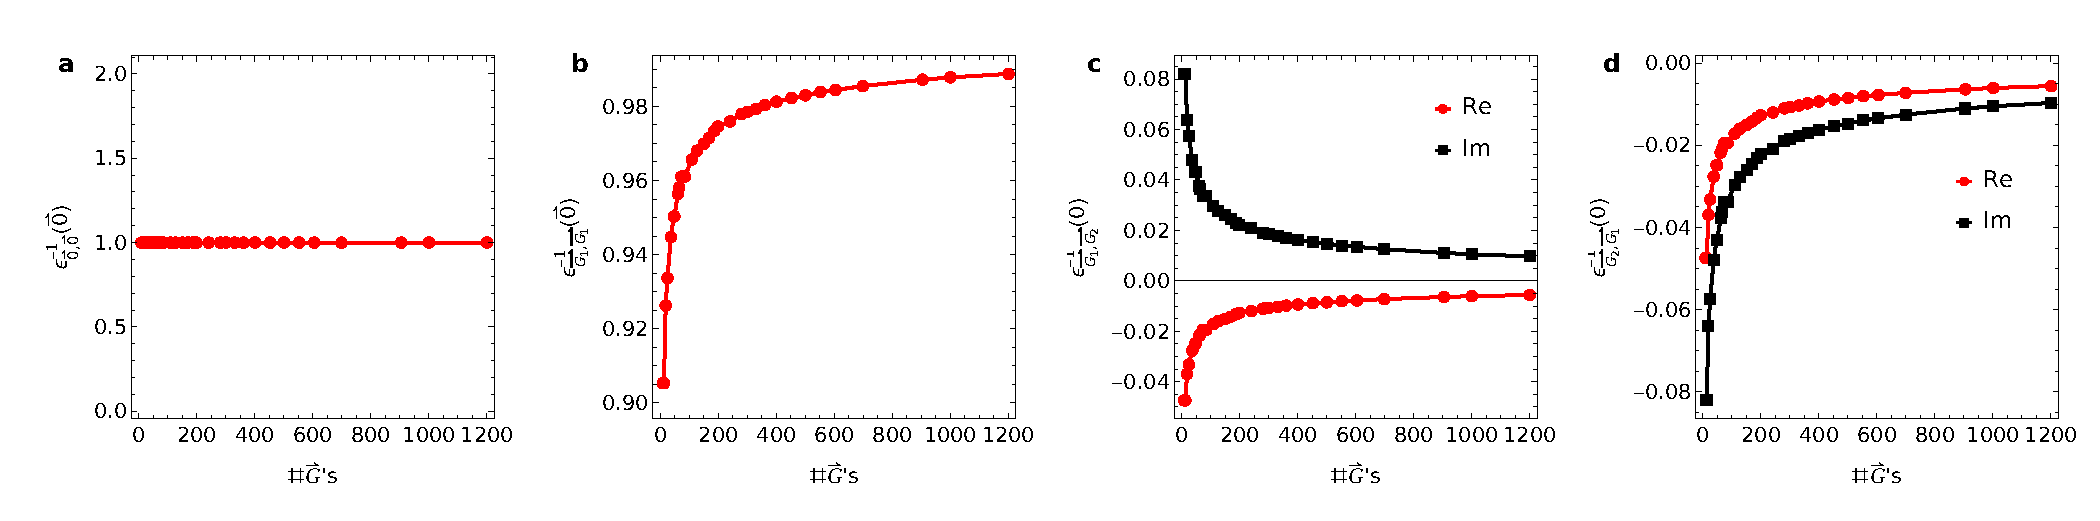
\includegraphics[width=1.0\linewidth]{Figures/epsilonInv_q0_row.pdf}
    \caption{Selection of matrix elements $\varepsilon^{-1}_{\bG \bG'} (\bzero)$ for \ch{MoS2} using Ridolfi's tight-binding model. All bands included, and with a BZ mesh with 20 momentum points in each direction. \textbf{a} $(\bG,\bG') = (\bzero,\bzero)$, \textbf{b} $(\bG,\bG') = (\bG_1,\bG_1)$, \textbf{c} $(\bG,\bG') = (\bG_1,\bG_2)$, \textbf{d} $(\bG,\bG') = (\bG_2,\bG_1)$. $\bG_1 = (-1.98835, 1.14797)$(\AA$^{-1}$)  and $\bG_2 = -\bG_1$.}
\end{figure}
    
\end{frame}

\begin{frame}{Macroscopic dielectric function}

\begin{columns}

\column{0.2\textwidth}

\onslide<1->{
\begin{equation*}
    \varepsilon_{\text{2D}}(\bq) \equiv \frac{1}{\varepsilon^{-1}_{\bzero \bzero}(\bq)}
\end{equation*}

\begin{equation*}
    \varepsilon_{\text{RK}}(\bq) = 1 + r_0 q
\end{equation*}
}


\column{0.8\textwidth}

\onslide<2->{
\begin{figure}[H]
    \centering
    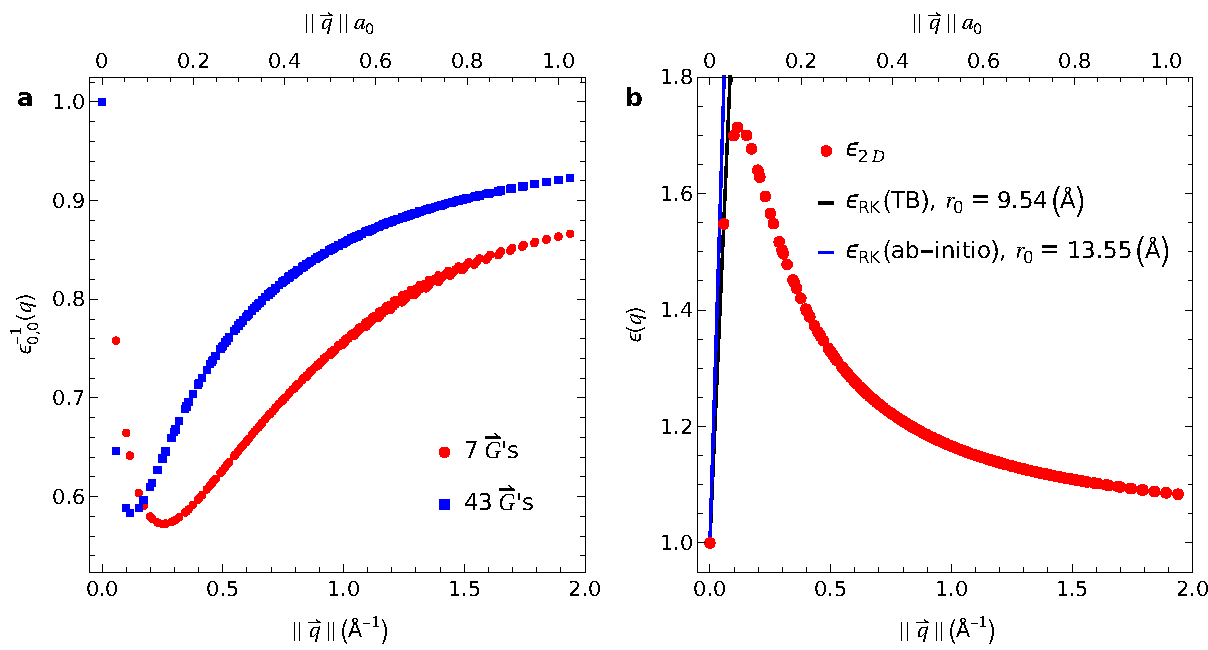
\includegraphics[width=0.8\linewidth]{Figures/epsilonvsq_comparison.pdf}
    \caption{\textbf{a} $\varepsilon^{-1}_{\bzero \bzero}(|\bq|)$ and \textbf{b} $ \varepsilon_{\text{2D}}(|\bq|)$. For \ch{MoS2} using Ridolfi's tight-binding model. In \textbf{b} we display the numerical $\varepsilon_{\text{2D}}$, the Rytova-Keldysh dielectric function with an estimated $r_0 \approx 9.54$ \AA \,and with the ab-initio one $r_0=13.55$ \AA.}
\end{figure}}

\end{columns}

    
\end{frame}

\begin{frame}{Screened potential}


\begin{columns}[T]

\column{0.5\textwidth}

\onslide<1->{
\begin{equation*}
    v_c(\bq) = \frac{e^2}{2 \varepsilon_0 q} \onslide<2->{\,\text{\textcolor{black}{(black dots)}}}
\end{equation*}
%\vspace{-0.3cm}
\begin{equation*}
    V_{\text{RK}}(\bq) = \frac{e^2}{2 \varepsilon_0 (1 + r_0 q)q}\onslide<2->{\,\text{\textcolor{blue}{(blue dots)}}}
\end{equation*}
%\vspace{-0.3cm}
\begin{equation*}
    W_{\bzero \bzero}(\bq) = \varepsilon^{-1}_{\bzero \bzero}(\bq) v_c(\bq)\onslide<2->{\,\text{\textcolor{red}{(red dots)}}} 
\end{equation*}
%\vspace{-0.3cm}

}

\only<3->{
\begin{itemize}
    \item $W_{\bzero \bzero}(\bq) \xrightarrow{q \nearrow} v_c(\bq)$ \itemsep=2.5em
    \item RK approx. overestimates screening 
\end{itemize}

}

\column{0.5\textwidth}

\onslide<2->{
\vspace{-0.5cm}
\begin{figure}[H]
    \centering
    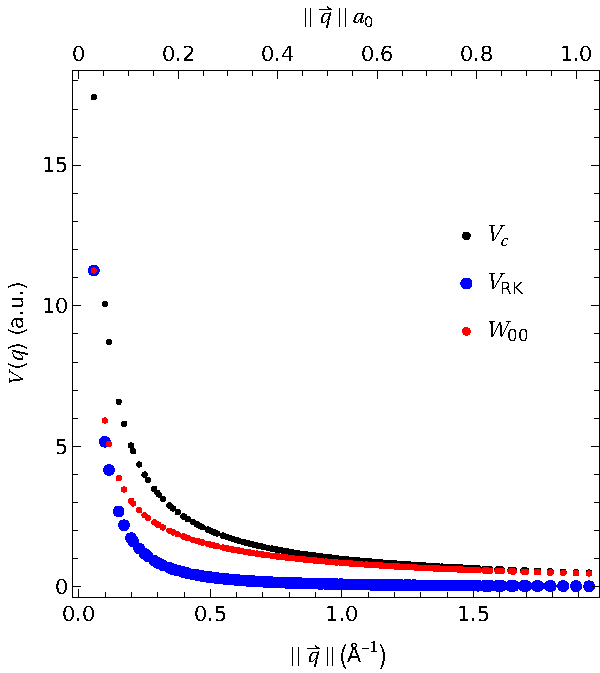
\includegraphics[scale=0.55]{Figures/Vvsq.pdf}
    \caption{Bare and screened potentials for \ch{MoS2} using Ridolfi's TB model. 43 $\bG$s included.}
    \label{fig:potentials_comparison}
\end{figure}}


\end{columns}

\end{frame}

\begin{frame}{A use case: excitons in \ch{MoS2}}

Please consult: Alejandro José Uría-Álvarez et al. “Efficient computation of optical excitations in 2D materials with the Xatu code”, Computer Physics Communications 295 (2024)

\begin{table}[ht]
\begin{tabular}{|c|c|c|c|c|}
\hline
\multicolumn{1}{|l|}{State} & \multicolumn{1}{l|}{Energy (RK) (eV)} & \multicolumn{1}{l|}{B. energy (RK) (eV)} & \multicolumn{1}{l|}{Energy ($\varepsilon_{\bG,\bG'}$) (eV)} & \multicolumn{1}{l|}{B. energy ($\varepsilon_{\bG,\bG'}$) (eV)} \\ \hline
1a                          & \multirow{2}{*}{1.15051}              & \multirow{2}{*}{-0.96949}                     & 0.858549                                                    & -1.261451                                                           \\ \cline{1-1} \cline{4-5} 
1b                          &                                       &                                               & 0.858551                                                    & -1.261449                                                           \\ \hline
2a                          & \multirow{2}{*}{1.187938}             & \multirow{2}{*}{-0.932062}                    & 0.900934                                                    & -1.219066                                                           \\ \cline{1-1} \cline{4-5} 
2b                          &                                       &                                               & 0.900936                                                    & -1.219064                                                           \\ \hline
3a                          & \multirow{2}{*}{1.266467}             & \multirow{2}{*}{-0.853533}                    & 0.971518                                                    & -1.148482                                                           \\ \cline{1-1} \cline{4-5} 
3b                          &                                       &                                               & 0.971520                                                    & -1.14848                                                            \\ \hline
4a                          & \multirow{2}{*}{1.305554}             & \multirow{2}{*}{-0.814446}                    & 1.015683                                                    & -1.104317                                                           \\ \cline{1-1} \cline{4-5} 
4b                          &                                       &                                               & 1.015685                                                    & -1.104315                                                           \\ \hline
\end{tabular}
\caption{Exciton spectrum of \ch{MoS2} described by Ridolfi's tight-binding model, using the Rytova-Keldysh potential and the computed inverse dielectric matrix to compute the interaction matrix elements, at the left and right, respectively. $N_k=40^2$, $N_c=N_v=2$ for the exciton, $N_G=43$. Excludes the exchange interaction term in both approaches to screening.}
\end{table}
    
\end{frame}

%%%%%%%%%%%%%%%%%%%%%%%%%%%%%%%%%%%%%%%%%%%%%%%%%%

\section{What is in order? Real space approach}

%%%%%%%%%%%%%%%%%%%%%%%%%%%%%%%%%%%%%%%%%%%%%%%%%%%

\begin{frame}{Outline}
  \tableofcontents
\end{frame}



\begin{frame}{Revisiting Dyson's equation}

\begin{equation*}
\label{eq:polarizability_RPA_Bloch_states}
    \chi_0 (\br,\br';\omega) = \sum_{v \bk, c\bk'} \left[ \frac{\psi_{c \bk'}(\br) \psi_{v \bk}^*(\br) \psi_{v \bk}(\br') \psi_{c \bk'}^*(\br') }{\hw -(\epsilon_{c \bk'} - \epsilon_{v \bk})   + \ii \hbar \alpha} - \frac{ \psi_{v \bk}(\br) \psi_{c \bk'}^*(\br) \psi_{c \bk'}(\br') \psi_{v \bk}^*(\br') }{\hw + (\epsilon_{c \bk'} - \epsilon_{v \bk}) + \ii \hbar \alpha} \right]\,.
\end{equation*}

\begin{equation*}
    W(\br,\br') = \int \dr'' \varepsilon^{-1} (\br,\br'') v_c (\br'',\br') = v_c (\br,\br') + \int \dx \int \dy\, v_c (\br,\bx) \chi_0 (\bx,\by) W(\by,\br')
\end{equation*}

\begin{equation*}
    \psi_{n \bk} (\br) = \frac{1}{\sqrt{N}} \sum_{\bR} \ee^{\ii \bk \cdot \bR} \sum_{i \alpha} C_{i \alpha}^{n \bk} \phi_{\alpha} (\br - \bR - \bt_i),
\end{equation*}

    
\end{frame}

\begin{frame}{Revisiting Dyson's equation}

In the continuum

\begin{equation*}
    W(\br,\br') = \int \dr'' \varepsilon^{-1} (\br,\br'') v_c (\br'',\br') = v_c (\br,\br') + \int \dx \int \dy\, v_c (\br,\bx) \chi_0 (\bx,\by) W(\by,\br')
\end{equation*}

Discretized version, in the point-like orbital approximation

\begin{equation*}
    W(\bR + \bt_i,\bt_j) = v_c (\bR + \bt_i,\bt_j) + \sum_{i',\bR_1}^{\bR_1+\bt_{i'} \neq \bR+\bt_i}  v_c (\bR + \bt_{i},\bR_1 + \bt_{i'}) \sum_{j',\bR''}^{\bR''+\bt_{j'} \neq \bt_j} \mathcal{T}^{i',j'}_{\bR_1,\bR''} W(\bR'' + \bt_{j'},\bt_j)
\end{equation*}

\begin{equation*}
    \mathcal{T}^{i,j}_{\bR,\bR'} \equiv \frac{1}{N^2} \sum_{v \bk, c\bk'} \sum_{\alpha \beta} \frac{-2 \Re{(C^{c \bk'}_{i \alpha})^* C^{v \bk}_{i \alpha} (C^{v \bk}_{j \beta})^* C^{c \bk'}_{j \beta} \ee^{-\ii (\bk' - \bk) \cdot (\bR - \bR')} }}{\epsilon_{c \bk'} - \epsilon_{v \bk}}
\end{equation*}
    
\end{frame}

\begin{frame}{Screened potential in real space}

\begin{equation*}
    W(\bR + \bt_i,\bt_j) = v_c (\bR + \bt_i,\bt_j) + \sum_{i',\bR_1}^{\bR_1+\bt_{i'} \neq \bR+\bt_i}  v_c (\bR + \bt_{i},\bR_1 + \bt_{i'}) \sum_{j',\bR''}^{\bR''+\bt_{j'} \neq \bt_j} \mathcal{T}^{i',j'}_{\bR_1,\bR''} W(\bR'' + \bt_{j'},\bt_j)
\end{equation*}

 is equivalent to


\begin{equation*}
     \hspace*{-0.55cm}W(\bR + \bt_i,\bt_j) - \sum_{j',\bR''}^{\bR''+\bt_{j'} \neq \bt_j} \left[ \sum_{i',\bR_1}^{\bR_1+\bt_{i'} \neq \bR + \bt_i} v_c (\bR + \bt_{i},\bR_1 + \bt_{i'}) \mathcal{T}^{i',j'}_{\bR_1,\bR''}  \right] W(\bR'' + \bt_{j'},\bt_j)  = v_c (\bR + \bt_i,\bt_j)
\end{equation*}

System of linear equations, however....

\begin{itemize}
    \item $W(\bR + \bt_i,\bt_j) > 0$ sometimes, $W(\bR + \bt_i,\bt_j) < 0$ other times;
    \item Situation improves including the term $\bR_1+\bt_{i'} = \bR + \bt_i$, but result is regularization dependent.
\end{itemize}
    
\end{frame}

\begin{frame}{Screened potential in real space: what to do?}

\begin{itemize}
    \item Look at what chemists do.
    \item Self-consistent approach? \\ $W(\bR + \bt_i,\bt_j) = v_c (\bR + \bt_i,\bt_j) + \sum_{i',\bR_1}^{\bR_1+\bt_{i'} \neq \bR+\bt_i}  v_c (\bR + \bt_{i},\bR_1 + \bt_{i'}) \sum_{j',\bR''}^{\bR''+\bt_{j'} \neq \bt_j} \mathcal{T}^{i',j'}_{\bR_1,\bR''} v_c(\bR'' + \bt_{j'},\bt_j) + ....$
\end{itemize}

\begin{figure}[H]
    \centering
    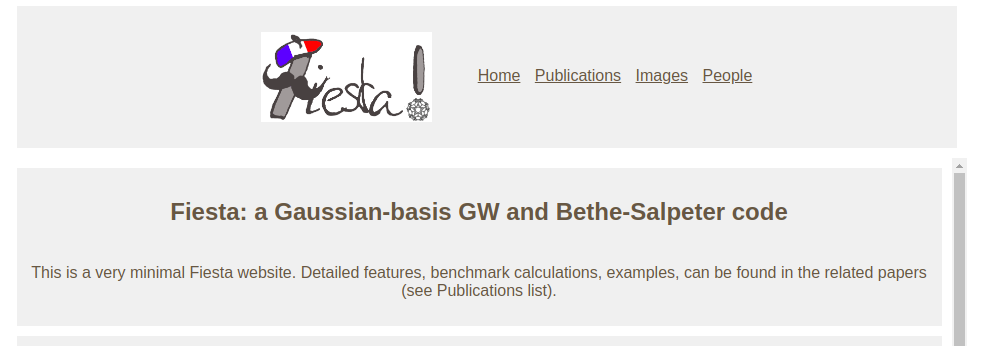
\includegraphics[scale=0.25]{Figures/Fiesta.png}
\end{figure}
    
\end{frame}



\begin{frame}{Acknowledgments}

\only<1->{
\begin{textblock*}{4.0cm}(2.5cm,1.0cm)
\centering
Juan José Palácios
\begin{figure}
    \centering
    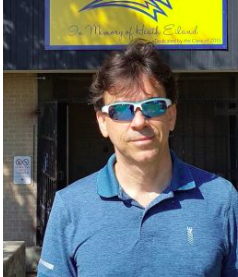
\includegraphics[scale=0.3]{Figures/Palacios.png}
\end{figure}
\end{textblock*}

\begin{textblock*}{4.0cm}(-.3cm,5cm)
\centering
Alex
\begin{figure}
    \centering
    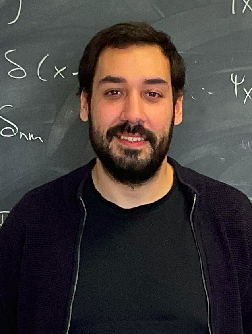
\includegraphics[scale=0.22]{Figures/Alex.png}
\end{figure}
\end{textblock*}}

\only<2->{
\begin{textblock*}{4.0cm}(2.5cm,5cm)
\centering
Juanjo
\begin{figure}
    \centering
    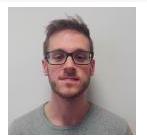
\includegraphics[scale=0.3]{Figures/Juanjo.png}
\end{figure}
\end{textblock*}

\begin{textblock*}{4.0cm}(2.5cm,8cm)
\centering
Simran
\end{textblock*}

\begin{textblock*}{4.0cm}(5.5cm,8cm)
\centering
David
\end{textblock*}

\begin{textblock*}{4.0cm}(5.5cm,5cm)
\centering
Manuel António
\begin{figure}
    \centering
    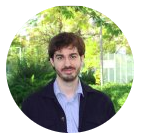
\includegraphics[scale=0.4]{Figures/Toni.png}
\end{figure}
\end{textblock*}}

\only<3->{
\begin{textblock*}{4.0cm}(9.5cm,1.0cm)
\centering
António Picón
\begin{figure}
    \centering
    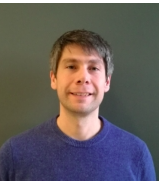
\includegraphics[scale=0.4]{Figures/AntonioPicon.png}
\end{figure}
\end{textblock*}

\begin{textblock*}{4.0cm}(8.5cm,5cm)
\centering
Miguel
\begin{figure}
    \centering
    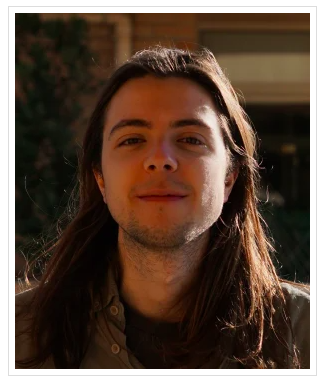
\includegraphics[scale=0.2]{Figures/Miguel.png}
\end{figure}
\end{textblock*}

\begin{textblock*}{4.0cm}(11.5cm,5cm)
\centering
Maurício
\begin{figure}
    \centering
    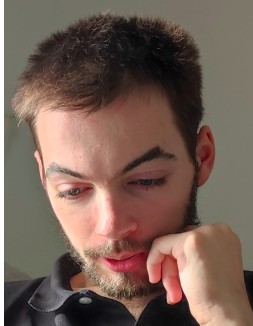
\includegraphics[scale=0.23]{Figures/Mauricio.png}
\end{figure}
\end{textblock*}}

\only<4->{
\begin{textblock*}{4.0cm}(-.3cm,1.cm)
\centering
Vinicius
\begin{figure}
    \centering
    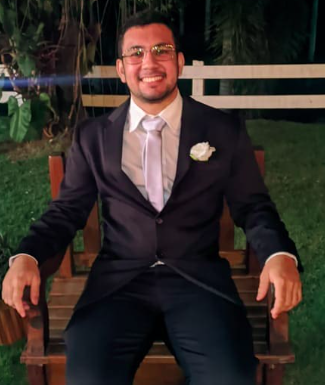
\includegraphics[scale=0.2]{Figures/Vinicius.png}
\end{figure}
\end{textblock*}

\begin{textblock*}{4.0cm}(6cm,1.cm)
\centering
Guilherme
\begin{figure}
    \centering
    
\includegraphics[scale=0.15]{Figures/Guilherme.png}
\end{figure}
\end{textblock*}
}

\only<5->{
\begin{textblock*}{4.0cm}(12.0cm,1.cm)
\centering
Johan
\begin{figure}
    \centering
    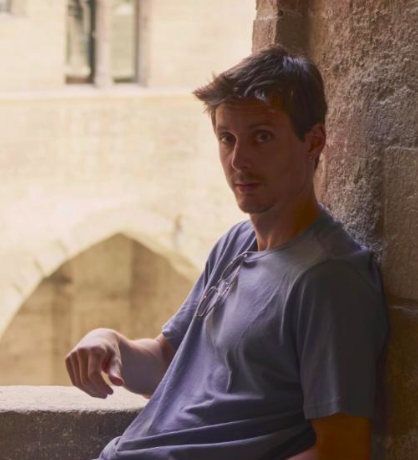
\includegraphics[scale=0.15]{Figures/Johan.png}
\end{figure}
\end{textblock*}
}


    
\end{frame}


\end{document}
